\subsection{Time-series Dense Encoder}
\textbf{TiDE} (Time-series Dense Encoder) là một mô hình dự báo chuỗi thời gian. Mô hình mã hóa chuỗi thời gian quá khứ cùng với hiệp phương sai bằng cách sử dụng “dense MLP” (Multi-Layer Perceptron). Sau đó, mô hình giải mã (decode) chuỗi thời gian được mã hóa (encode) cùng với các hiệp phương sai trong tương lai.
\begin{figure}[h]
    \centering
    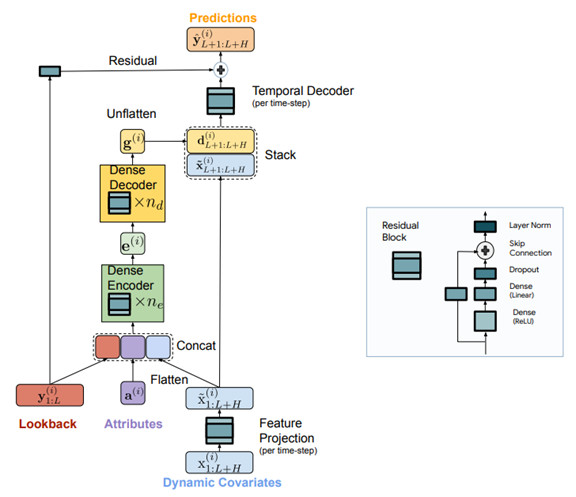
\includegraphics[width=0.5\textwidth]{img/TiDE.png}
    \caption{Tổng quan về kiến trúc TiDE}
    \label{fig:your_figure_label}
\end{figure}

\text{Kiến trúc tổng quan được trình bày ở Hình 4.} Đầu vào (input) của mô hình là dữ liệu quá khứ và phương sai của một chuỗi thời gian tại một thời điểm ($y_{1:L}^{(i)}, x_{1:L}^{(i)}, a^{(i)}$) và ánh xạ tới dự đoán của chuỗi thời gian $\hat{y}_{L+1:L+H}^{(i)}$.

\textbf{Residual Block:} Là một thành phần quan trọng của kiến trúc TiDE vì nó cho phép mô hình nắm bắt các tính chất phi tuyến tính vốn có trong dữ liệu chuỗi thời gian, đồng thời duy trì các mối quan hệ tuyến tính nhằm giúp cải thiện hiệu suất dự báo dài hạn. 

Giả sử đầu vào của Residual Block là \( \mathbf{x} \), công thức của nó có thể được mô tả như sau:

\begin{itemize}
    \item Layer Normalization:
    \[
    \mathbf{h}_0 = \text{LayerNorm}(\mathbf{x})
    \]

    \item Lớp Dense đầu tiên với ReLU Activation:
    \[
    \mathbf{h}_1 = \text{ReLU}(\mathbf{W}_1 \mathbf{h}_0 + \mathbf{b}_1)
    \]

    \item Dropout (tùy chọn):
    \[
    \mathbf{h}_1 = \text{Dropout}(\mathbf{h}_1, p)
    \]
    Trong đó, \( p \) là xác suất giữ lại của Dropout.

    \item Lớp Dense thứ hai:
    \[
    \mathbf{h}_2 = \mathbf{W}_2 \mathbf{h}_1 + \mathbf{b}_2
    \]

    \item  ReLU Activation sau Kết nối tắt (Skip Connection):
    \[
    \tilde{\mathbf{x}} = \text{ReLU}(\mathbf{x} + \mathbf{h}_2)
    \]

\end{itemize}

Trong đó:
\begin{itemize}
    \item \( \mathbf{W}_1 \) và \( \mathbf{W}_2 \) là các ma trận trọng số của các lớp Dense MLP.
    \item \( \mathbf{b}_1 \) và \( \mathbf{b}_2 \) là các vector bù.
    \item \(\text{LayerNorm}(\cdot)\) là hàm chuẩn hóa lớp.
    \item \(\text{Dropout}(\cdot, p)\) là hàm Dropout với xác suất \( p \).
    \item \(\text{ReLU}(\cdot)\) là hàm kích hoạt ReLU.
    \item \(\tilde{\mathbf{x}}\) là đầu ra của Residual Block.
\end{itemize}

\textbf{Mã hóa (Encoding):}
\begin{itemize}
    \item \textbf{Feature Projection:} Sử dụng residual block để ánh xạ \( x_t^{(i)} \) tại mỗi time-step, hoạt động này được mô tả như sau:
    \[
        \tilde{x}_t^{(i)} = \text{ResidualBlock}(x_t^{(i)}) 
    \]

    \item \textbf{Dense Encoder:} Xếp chồng và làm phẳng tất cả các biến động trong quá khứ và tương lai, nối chúng với các thuộc tính tĩnh và quá khứ của chuỗi thời gian. Ánh xạ vào một embedding bằng cách sử dụng một bộ mã hóa chứa nhiều khối dư:
    \[
    e^{(i)} = \text{Encoder}\left( y_{1:L}^{(i)}, \tilde{x}_{1:L}^{(i)}, \tilde{x}_{1:L+H}^{(i)}, a^{(i)} \right)
    \]
\end{itemize}

\textbf{Giải mã (Decoding):}

\begin{itemize}
    \item \textbf{Dense Decoder (Bộ giải mã dense):} Đơn vị giải mã đầu tiên xếp chồng nhiều khối dư giống bộ mã hóa với cùng kích thước lớp ẩn, nhận đầu vào là mã hóa \( e^{(i)} \), ánh xạ thành vector \( g^{(i)} \) kích thước \( H \times p \) (\texttt{decoderOutputDim}), và chuyển đổi thành ma trận \( D^{(i)} \in \mathbb{R}^{p \times H} \):
    \[
    g^{(i)} = \text{Decoder}(e^{(i)}) \in \mathbb{R}^{p \times H}
    \]
    \[
    D^{(i)} = \text{Reshape}(g^{(i)}) \in \mathbb{R}^{p \times H}
    \]

    \item \textbf{Temporal Decoder (Bộ giải mã thời gian):} Cuối cùng, bộ giải mã thời gian, một khối dư với đầu ra kích thước 1, ánh xạ vector \( d^{(i)}_t \) tại thời điểm \( t \) kết hợp với các phương sai đã được chiếu \( \tilde{x}^{(i)}_{L+t} \):
    \[
    \hat{y}^{(i)}_{L+t} = \text{TemporalDecoder}(d^{(i)}_t, \tilde{x}^{(i)}_{L+t}) \quad \forall t \in [H]
    \]
\end{itemize}